\chapter{Alta disponibilidade}

\section{Definição da alta disponibilidade}

Alta disponibilidade é bastante conhecida, sendo cada vez mais empregada nos ambientes computacionais.
O objetivo de promover alta disponibilidade resume-se em um serviço estar sempre 
a disposição quando o cliente solicitar ou acessar \cite{costa2009}.
Pode-se definir alta disponibilidade como a redundância de \textit{hardware} ou \textit{software} para que o serviço fique mais tempo disponível.
Quanto maior for a disponibilidade desejada maior deverá ser a redundância no ambiente, assim reduzindo os pontos únicos de falha,
em inglês \textit{Single Point Of Failure} (SPOF).

A alta disponibilidade está diretamente relacionada a dependabilidade, confiabilidade, disponibilidade e tolerância a falhas. 

A dependabilidade indica a qualidade do serviço fornecido e a confiança depositada nele. A dependabilidade envolve vários
atributos como confiabilidade, disponibilidade, segurança, entre outros. Os atributos mais relevantes são confiabilidade e disponibilidade 
\cite{weber2002}.

A confiabilidade, é o mais importante atributo, pois transmite a ideia de continuidade de serviço \cite{pankaj1994}. Confiabilidade refere-se 
a probabilidade de um serviço funcionar corretamente durante um dado intervalo de tempo. Já a disponibilidade é a probabilidade de um 
serviço estar operacional no instante em que for solicitado \cite{costa2009}.

Por sua vez a tolerância a falhas fornece disponibilidade de um serviço utilizando mecanismos capazes de detectar, mascarar e recuperar falhas, 
e seu objetivo é alcançar a dependabilidade, assim indicando uma boa qualidade de serviço \cite{costa2009}.
Uma das principais palavras-chave da alta disponibilidade é a tolerância a falhas, que será melhor detalhada na próxima seção.

\section{Tolerância a falhas}

Sabe-se que o \textit{hardware} tende a falhar por isso utiliza-se métodos como prevenção de falhas e tolerância a falhas.
A abordagem prevenção de falhas melhora a disponibilidade e a confiabilidade de um serviço porém, não resolverá todas as possíveis falhas.
Sendo assim, a tolerância a falhas fornece disponibilidade de um serviço mesmo com presença de falhas \cite{pankaj1994}.
O objetivo da tolerância a falhas é aumentar a disponibilidade de um sistema, isto é, aumentar o tempo que os serviços fornecidos aos 
clientes ou usuários ficam disponíveis. Um sistema é dito tolerante a falhas se ele pode mascarar a presença de falhas 
ou recuperar-se de uma falha, frenquentemente a tolerância a falhas é implementada utilizando redundância detalhada na próxima seção.

A tolerancia a falhas pode ser dividida em duas classes:
\begin{itemize}
 \item Mascaramento;
 \item Detecção, localização e reconfiguração.
\end{itemize}

Na primeira classe o mascaramento trata as falhas na origem e manifesta-se na forma de erro. Um exemplo são os 
códigos de correção de erros, em inglês \textit{error correction code} (ECC), utilizados em memórias para detecção e correção de erros.
Na segunda, geralmente necessita de menor redundância, e consiste em detectar, localizar e reconfigurar o \textit{software} ou
\textit{hardware} e por fim resolver a falha \cite{weber2002}.

\subsection{Fases da tolerância a falhas}

A classificação das fases de tolerância a falhas mais comuns são detecção, confinamento, recuperação e tratamento. Essas fases excluem
o mascaramento de falhas \cite{weber2002}.

\begin{figure}[falhasrecup]
 \centering
 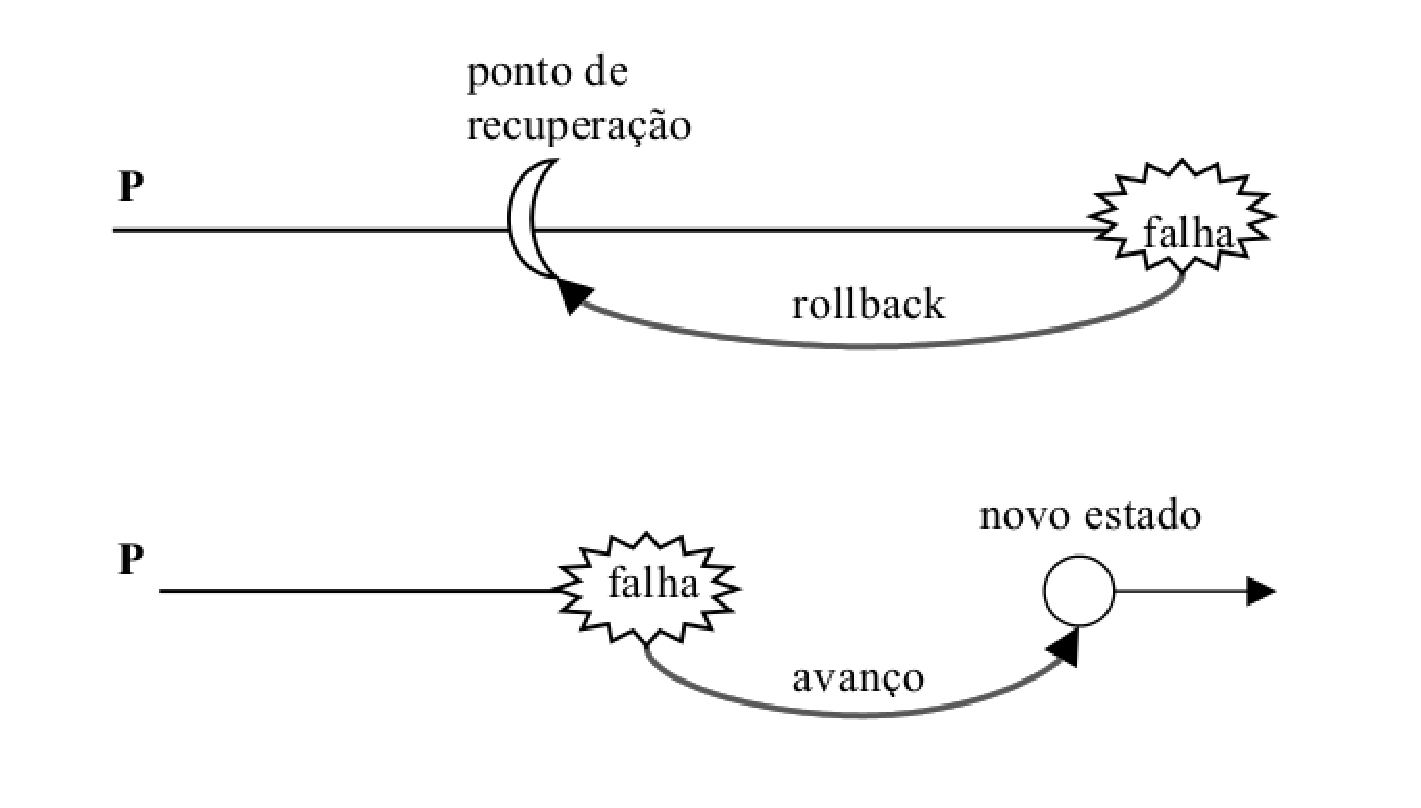
\includegraphics[height=200px]{img/recuperacao_ret_ava.eps}
 \caption{Recuperação por retorno e por avanço.}
 \label{fig:recuperacao_ret_ava}
\end{figure}

\begin{itemize}
 \item Detecção: é a primeira fase, a detecção de erro faz o monitoramento e aguarda uma falha se manifestar na forma de erro, para então
 passar para a próxima fase. Um exemplo de detecção de erro é o esquema de duplicação e comparação, que é a replicação de um componente
 que realiza as mesmas operações sobre os mesmos dados e compara os resultados de saída. Caso ocorra alguma diferença um erro é gerado.
 \item Confinamento: esta fase é reponsável pela restrição de um erro para não se propagar para todo o sistema, pois entre a falha e a
 detecção do erro há um intervalo de tempo. Onde pode ocorrer a propagação do erro para outros componentes do sistema, por isso antes de
 executar medidas corretivas é necessário definir limites da propagação.
 \item Recuperação: Após a detecção de um erro ocorre a recuperação, onde o estado de erro é alterado para estado livre de erros. A recuperação
 pode ser feita de duas formas:
 \subitem \textit{forward error recovery} ou recuperação por avanço, condução para um novo estado não ocorrido anteriormente. É o mais eficiente, 
 porém complexo de ser implementado pois a ação deve ser precisa. Ilustrado no segundo item da \ref{fig:recuperacao_ret_ava}.
 \subitem \textit{backward error recovery} ou recuperação por retorno, ocorre um retorno para um estado anterior que deve estar livre de erros.
 Para retornar ao estado anterior pode ser utilizado pontos de recuperação (\textit{checkpoints}), e quando ocorrer um erro, um \textit{rollback} 
 é executado, assim retornará ao \textit{checkpoint} anterior, conforme \ref{fig:recuperacao_ret_ava}.
 \item Tratamento: A última fase serve para prevenir que futuros erros aconteçam. Inicia com a localização da falha para encontrar o componente
 que originou a falha, após é feito um diagnóstico, que testa o componente e compara o resultado gerado com o previsto. Então o componente 
 danificado é removido, pode ser feito de duas formas, manual ou automático. O reparo manual é feito por operador, e o automático quando existe
 um componente em espera para substituição. Exemplo de um reparo manual é a troca de um disco de um servidor, e automático uma substituição
 de um componente de um satélite que possui longo período sem contato com algum operador.
\end{itemize}

\section{Redundância}

Redundância pode ser feita através da replicação de componentes, para reduzir o número de SPOF e garantir o mascaramento de falhas.
Na prática, se um componente falhar ele deve ser reparado ou substituido por um novo sem que haja uma interrupção no serviço.
Também pode ser através do envio de sinais ou \textit{bits} de controle junto aos dados, 
servindo assim para detecção de erros e até para correção \cite{weber2002}.

Segundo \cite{norvag2000} existem quatro tipos diferentes de redundância que são:
\begin{itemize}
 \item \textit{Hardware}: utiliza-se replicação de componentes, sendo que caso um falhe outro possa assumir seu lugar. 
 Para fazer a detecção de erros a saída de cada componente é constantemente monitorada e comparada à saída de outros componentes.
 Um exemplo prático de redundância de \textit{hardware} é servidores com fontes redundantes, normalmente são duas fontes ligadas em paralelo, 
 caso uma falhe a outra suprirá a necessidade de todo o servidor;
 \item Informação: quando uma informação extra é enviada ou armazenada para possibilitar a detecção e correção de erros.
 Um exemplo clássico são os \textit{checksums}, soma de verificação, é calculado a soma dos dados antes da transmissão ou armazenamento 
 e recalculado ao recebê-los ou recuperá-los, assim sendo possível verificar a integridade dos dados. Outro exemplo bastante comum são os 
 \textit{bits} de paridade, são utilizandos para detectar falhas simples, que afetam apenas um \textit{bit}. O \textit{bit} de paridade 
 serve apenas para checar se em um conjunto de n \textit{bits} existe um número par de zeros (ou número ímpar dependendo do tipo de paridade 
 utilizado) \cite{weber2002};
 \item \textit{Software}: são todos os \textit{softwares} ou instruções utilizados para suporte a tolerância a falhas. Podem ser implementados
 de várias formas, desde um processo que fica monitorando o serviço para verificar se ele está funcionando corretamente, até um programa
 que efetua uma verificação nos resultados para saber se está operando da forma desejada. Exemplo de redundância de \textit{software} são 
 blocos de recuperação, que funcionam com um programa primário e um ou mais programas secundários, caso o programa primário falhar um secundário
 entrará em seu lugar;
 \item Tempo: este é feito através da execução de instruções várias vezes no mesmo componente, assim detectando falha caso ocorra.
 Necessita tempo adicional, e é utilizado onde o tempo não é crítico. Por exemplo, um cão de guarda (\textit{watchdog timer})
 recebe um sinal do programa ou serviço monitorado e caso este sinal não seja recebido, devido alguma falha, o \textit{watchdog} irá fazer 
 uma ação de reinicialização do serviço.
 Diferentemente de redundância de \textit{hardware} e informação ela não requer um \textit{hardware} extra para sua implementação \cite{costa2009}.
\end{itemize}

\section{Cálculo da alta disponibilidade}

Um ponto importante sobre alta diponibilidade é como medi-la. Para isso são utilizados os valores de \textit{uptime} e 
\textit{downtime}, que são respectivamente o tempo que os serviços estão funcionando normalmente e o tempo que não estão funcionando.
Outra forma de expressar a alta disponibilidade é pela quantidade de ``noves'', isto é, se um serviço possui 4 noves de disponibilidade
este possui uma disponibilidade de 99,99\% \cite{pereirafilho2004}.

\begin{table}
\caption {Níveis de alta disponibilidade}
\label{tab:dispniveis} 
\begin{center}
\begin{tabular}{|l|l|l|l|}\hline
Nível & Uptime & Downtime por ano & Downtime por semana\\\hline
1 & 90\% & 36.5 dias & 16 horas e 51 minutos\\\hline
2 & 98\% & 7.3 dias & 3 horas e 22 minutos\\\hline
3 & 99\% & 3.65 dias & 1 hora e 41 minutos\\\hline
4 & 99.8\% & 17 horas e 30 minutos & 20 minutos e 10 segundos\\\hline
5 & 99.9\% & 8 horas e 45 minutos & 10 minutos e 5 segundos\\\hline
6 & 99.99\% & 52.5 minutos & 1 minuto\\\hline
7 & 99.999\% & 5.25 minutos & 6 segundos\\\hline
8 & 99.9999\% & 31.5 minutos & 0.6 segundos\\\hline
\end{tabular}
\end{center}
\end{table}

\begin{table}
\caption {Exemplos de sistemas e seus níveis de disponibilidade}
\label{tab:dispexemplos} 
\begin{center}
\begin{tabular}{|l|l|}\hline
Nível  & Nome\\\hline
1 & computadores pessoais\\\hline
3 & sistemas de acesso\\\hline
5 & provedores de internet\\\hline
6 & CPD, sistemas de negócios\\\hline
7 & sistemas de telefonia; sistemas de saúde; sistemas bancários\\\hline
8 & sistemas de defesa militar\\\hline
\end{tabular}
\end{center}
\end{table}

A tabela \ref{tab:dispniveis} possui alguns níveis de disponibilidade enumerados, seguido da porcentagem do \textit{Uptime}, 
o \textit{Downtime} por ano representado na medida de tempo, e o \textit{Downtime} por semana também na medida de tempo. 
Já a Tabela \ref{tab:dispexemplos} possui alguns exemplos de serviços relacionados ao nível de disponibilidade da tabela anterior. 
Pode-se observar que para alguns serviços como sistemas bancários ou sistemas militares é necessário um alto nível de disponibilidade.

Podemos calcular a disponibilidade através da equação
\begin{equation}
d = \frac{MTBF}{(MTBF + MTTR)}
\label{diponibilidade}
\end{equation}
onde $d$ é a porcentagem de disponibilidade. O \textit{Mean Time Between Failures} ($MTBF$) é o tempo médio entre falhas, correspondente ao tempo médio 
entre as paradas dos serviços. E o \textit{Mean Time To Repair} ($MTTR$) é o tempo médio de recuperação, isto é, o tempo 
entre a queda e a recuperação de um serviço \cite{goncalves2009}.

A alta disponibilidade é um dos principais fatores para garantir a confiança de clientes ou usuários, principalmente para empresa que 
fornece serviços \textit{on-line}. Por isso existe o \textit{Service Level Agreement} (SLA), acordo de nível de serviço, 
que garante que o serviço fornecido atenda as expectativas \cite{smith2010}. DETALHAR, ONDE?


%\textit{Software} não possui falhas causadas por fatores físicos, ao contrário de \textit{hardware}.
%Falhas em \textit{software} são causadas por erros no seu desenvolvimento, resultando assim em ``\textit{bugs}'' que geralmente
%são causados por erros humanos. 
